% !TeX root = main.tex
% !TeX spellcheck = en-US
% !TeX encoding = utf8


\chapter{Implementation}
\label{chap:implementation}
\glsreset{hsppbo}
\glsreset{hpo}
\glsreset{bo}

\epigraph{A tool that does everything is optimized for nothing.}

\section{Modules}
\label{chap:modules}

The implementation used for all the experiments in this thesis combines several theoretical aspects from \cref{chap:background}. The foundation, of course, is the \gls{hsppbo} algorithm implemented as explained in \cref{chap:hsppbo}. Then a \gls{hpo} framework using \gls{bo} was built around this algorithm, along with several other modes of operation, that make use of the metaheuristic algorithm. Although, the package is mostly adaptable to other combinatorial problem types, it has some aspects to it, that were designed with the \gls{dtsp} in mind. These are emphasized as such.

\begin{figure}[h]
	\centering
	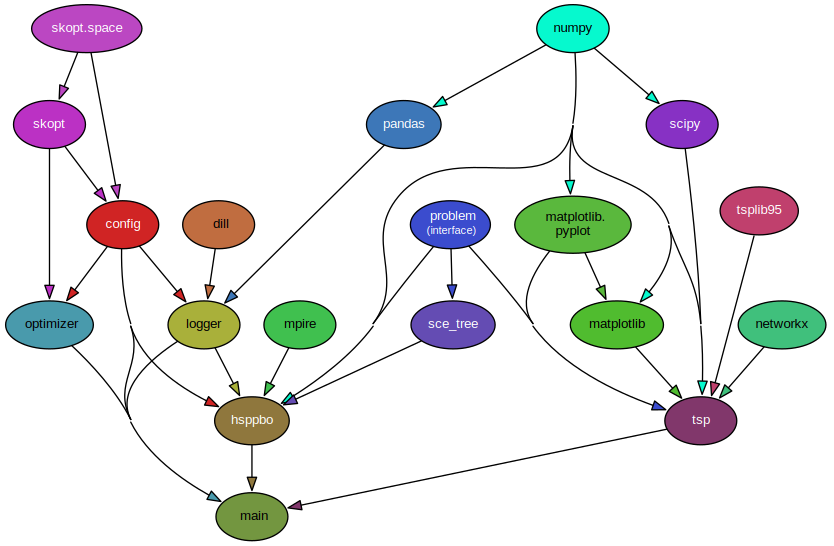
\includegraphics[width=0.95\textwidth]{code-dependency.svg}
	\caption{Dependency graph of the \textit{XF-OPT/META} python software package}
	\label{fig:dependency}
\end{figure}

The entire program package was written in \textit{Python}, with some modules completely imported from established libraries (especially for \gls{ml} and statistical functionality), some modules consisting of modified libraries that did not quite meet the requirements, and some completely new modules. \Cref{fig:dependency} shows the dependency graph starting from the \texttt{main} function, with a maximum depth of three references. 
These modules, their dependencies, and their general functionality are individually explained in the following subsections to provide a better understanding of the experiments and the research process.

\subsection{H-SPPBO Module}
\label{chap:hsppbo-module}
The \texttt{hsppbo} module implements a multiprocessing version of the \gls{hsppbo} algorithm (see \ref{alg:hsppbo}). It is initialized using all the parameters discussed in \cref{chap:hsppbo}:
\begin{itemize}
	\item The three weights $w_{\text{persprev}}, w_{\text{persbest}}, w_{\text{parentbest}} \geq 0$ controlling the influence of their respective populations
	\item $\alpha, \beta \geq 0$ limiting the influence of the stochastic and the heuristic importance
	\item A detection threshold $\theta \in [0,1]$
	\item A categorical dynamic reaction type $H = \left\lbrace H_{\text{full}}, H_{\text{partial}}, \emptyset \right\rbrace$
	\item A number of iterations to pause detections for $L > 0$
	\item A maximum number of iterations $i_{\text{max}}$ (used as a termination criterion).
\end{itemize}

In addition, some parameters have been fixed in the code using the suggestions from the original paper \cite{kupfer2021hierarchical}. The number of \glspl{sce} is set to $|\mathcal{A}| = 13$ with three children per \gls{sce}. The weight for the random influence $w_\text{rand}$ is set to $\frac{1}{n-1}$ with $n$ being the dimension of the \gls{tsp} instance\footnote{This value might not be ideal for other problem types.}.

Since the algorithm is influenced by many random processes, it explicitly provides a function to manually set a random seed, i.e. every time a random number is drawn or something is chosen from a probability distribution, we can expect the same outcome. This not only makes personal benchmarking more comparable, but also allows reproducible solutions, which is a very important aspect in \gls{ml} research. The use of this feature for the experiments is discussed further in \cref{chap:testing}.

The solution construction process is implemented in a sequential, iterative manner, similar to the description around \cref{eq:hsppbo_prob}. An attempt to convert this task into a matrix computation problem, using the capabilities of the popular \textit{NumPy} \cite{harris2020array} library, resulted in worse or similar performance at best. Hence, this approach was not followed in order to reduce complexity.
As a result, the computational performance of the solution construction process relies heavily on the calculations of $s_{ik}(P)$, which is basically a lookup of a subset in an ordered set (see \cref{ex:subset}).
For this reason, a key-value hash-map (called \texttt{dictionary} in \textit{Python}) was used as the solution population $P$ and a write-once, read-many tuple was used for the potential subset. The crucial function is the following:
\begin{Listing}[h]
	\begin{minted}{python}
		
def is_solution_subset(subset: tuple, solution: dict) -> bool:
  try:
    return solution.get(subset[0]) + 1 == solution.get(subset[1])
  except:
    return False
	\end{minted}
	\caption{The \textit{Python} code for the check, if a set is a subset of an ordered subset.}
	\label{lst:subset}
\end{Listing}

This code works well for two important reasons.
First, in the case of the \gls{tsp}, the solution is essentially just a list of node identifiers of size $n$. Since these are the keys, the values are just their indices in this list.
Second, \texttt{dictionaries} have a great key lookup performance. The \texttt{get}-method returns the value of the given key.
Thus, using the first node of the subset as the dictionary key returns its index in the solution sequence. Therefore, adding one to this index and checking again for the index of the second node in the subset should result in equality, if the subset exists. 
Many other solutions have been tried, some not specific enough for this use case, others not focused on performance. This small function was the result of many optimization efforts and the complete creation process scales linearly with $n$. Every iteration, a total number of $|\mathcal{A}| = m$ solutions are created, which gives a worst case time complexity of $\mathcal{O}(n^m)$.

Other performance improvements are achieved through parallelization. During the solution creation and population update procedure, each \gls{sce} operates individually, with only the parent best solution as a reference. Therefore, this process is parallelized using the \texttt{mpire} library \cite{mpire2023} for problem dimensions $n > 100$. Smaller instances of the \gls{tsp} were sequentially fast enough to outperform their parallelized counterparts because the overhead to do so was greater than the gain in performance.

\subsubsection{SCE Tree Module}

The \glspl{sce}, their populations $P^A_{\text{persprev}}$,$P^A_{\text{persbest}}$ and the tree structure are encapsulated in their own module \texttt{sce\_tree}, which is an extensions of the $k$-ary tree package \texttt{treelib} \cite{chen2018treelib}.
We have separate classes for the tree (\texttt{SCETree}) and its nodes (\texttt{SCENode}). Each node is essentially an \gls{sce} $A \in \mathcal{A}$ and holds four variables:
\begin{itemize}
	\item $P^A_{\text{persprev}}$ (tuple): Previous solution of the SCE node
	\item $f(\mathbf{s}^A_{\text{persprev}})$ (float): Quality of the personal pervious solution
	\item $P^A_{\text{persbest}}$ (tuple): Personal best solution of the SCE node
	\item $f(\mathbf{s}^A_{\text{persbest}})$ (float): Quality of the personal best solution
\end{itemize}

The output of the solution quality function $f(\cdot)$ depends on the provided problem type and module, as well as the initialization of the solutions for the populations. This module and the specific case of the \gls{tsp} is explained in \cref{chap:impl-problem}.
After each \gls{sce} node is initialized, they are ordered into an $k$-ary tree, where $k = 3$ is the number of children each parent has. The structure is similar to \cref{fig:ternary-tree}.
The \texttt{treelib} base package already provides much of this functionality, but the swapping of the \glspl{sce} had to be implemented separately.
In addition, the algorithm-specific change handling procedures are also present in this module, either resetting the personal best solution of the whole tree ($H_{\text{full}}$) or only from the third level down ($H_{\text{partial}}$).

\subsection{Problem Interface}
\label{chap:impl-problem}

The \texttt{problem} module is implemented as an interface for all kinds of problem realizations. It uses \textit{Python}'s abstract methods to facilitate future development of other (dynamic) problem types, and provide guidance on all important methods, their parameters and return values. All other modules only use their problem instance through this interface, which further simplifies development.
Although the problem module should also contain the functions to validate, randomly generate, and evaluate its corresponding solutions, it does not store these solutions.

One of these problem types using the interface is the \texttt{tsp} module, which implements the symmetrical \gls{tsp} with optional dynamic capabilities to turn every instance into a \gls{dtsp} problem.

\subsubsection{TSP Module}
\label{chap:tsp-module}

The \texttt{tsp} module is a realization of the problem described in \cref{chap:tsp-theory}. Programmatically, it is based on the \texttt{tsplib95} library, which provides read, write, and transform functions for files in the \texttt{.tsp} file format proposed by \citet{reinelt1991tsplib}. It works very well with \gls{tsp} instances of the types \textit{EUC\_2D} (cities in a two-dimensional Euclidean space), \textit{GEO} (cities as geographic coordinates), and \textit{ATT} (special pseudo-Euclidean distance function), thus limiting the capabilities to these types.

The specific \gls{tsp} instance is initialized by its name (e.g., \texttt{rat195}) and then loaded by \texttt{tsplib95}. From this instance, the dimension $n$ is stored and the distance matrix $D$ is calculated using the package's Euclidean distance method and \texttt{numpy} \cite{harris2020array}.
Since all solutions generated by the \texttt{tsp} module are of the same type, they share a solution quality function $f : V^n \rightarrow \mathbb{R}_{0}^{+}$. It works as described in \cref{chap:hsppbo}, where each solution vector $\mathbf{s}$ is given as a $n$-dimensional combination of the solution space $V$, where the positive real value is the length of the traveled tour $L$.

The \gls{dtsp} is implemented by enabling the positional swap of two randomly selected city nodes.
This dynamic part of the problem is optional and can be initialized separately. The settings correspond to those of \citet{kupfer2021hierarchical} and are as follows:
\begin{itemize}
	\item A percentage $C \in [0,1]$ of how many cities $n$ are changing per dynamic turn
	\item A dynamic period $T_{d} \in \mathbb{N}$ defining how often the change is triggered
	\item A number of minimum iterations $i_{\text{min}}$ before the dynamic starts to trigger
\end{itemize}
That means, that starting from iteration $i_{\text{min}}$, every $T_{d}$ iterations ($i_{\text{min}} + k \cdot T_{d} < i_{\text{max}}, k \in \mathbb{N}$) a number of $\frac{n\cdot C}{2}$ distinct pairs of cities are randomly selected and swap their entries in the distance matrix $D$. After this procedure, the distance matrix is recalculated to reflect the changes.

To evaluate the problem instance itself, some statistical methods have been implemented. First, the length of the optimal solution to each symmetric \textit{TSPLIB} problem is stored in a metadata file. In addition to this information, the module can compute the mean and median distance of a problem, the standard deviation and the coefficient of variation for the distance, as well as the first eigenvalue, the \gls{cqv}, and a so-called regularity index according to \cite{clark1954distance, cricsan2021randomness, dry2012clustering}. More on the use of these values in \cref{chap:classification}.
Finally, the \gls{tsp} instances and their solutions can also be visualized using the \texttt{networkx} package \cite{hagberg2008exploring} (for an example, see \cref{fig:cluster-groups}).


\subsection{Optimizer Module}
\label{chap:optimizer}

Several options for the \gls{hpo} module were considered, but the requirements called for an adaptable library, that was not too closely tied to \gls{ml} application. Self-implementation was omitted early on to reduce complexity and potential for error. The libraries compared by \citet{yang2020hyperparameter} were reviewed and checked for potential use with metaheuristics. Ultimately, the \texttt{scikit-optimize} library \cite{head2020scikit} was chosen as the most versatile and adaptable option, while still providing reasonable performance. In addition to the basic \gls{rs} method, it also gives an implementation of \glsdesc{bo} with several options for surrogate models: \gls{gp}, \gls{rf}, \gls{et}, and \gls{gbrt} (see \cref{chap:bo} for details). And since \texttt{scikit-optimize} is built on top of the popular \gls{ml} library \texttt{scikit-learn} \cite{scikit-learn2011}, it allows other  regression models from that library to be used instead. Furthermore, it also provides three popular acquisition functions - \glsfirst{pi}, \glsfirst{ei} and lower confidence bound (LCB) - of which the two explained in \cref{chap:bo-acq} were used for the experiments of this thesis.
Overall, \texttt{scikit-optimize} provides the mature interfaces and development foundation of \texttt{scikit-learn}, while also implementing a customizable \glsdesc{bo} workflow.

Because of this already good base library, the actual implementation of the \texttt{optimizer} module only contains some interfaces to streamline the interaction between the metaheuristic (in this case \gls{hsppbo}) and the \gls{hpo} process. On initialization, the optimizer class needs only three things: 
First is the optimization algorithm to use. As mentioned earlier, these are \glsdesc{rs}, \glsdesc{rf}, \glsdesc{gp}, \glsdesc{rf}, \glsdesc{et}, and \glsdesc{gbrt}. However, the choice of acquisition function and other algorithm-specific parameters have been preconfigured or left default, depending on the algorithm, which is explained in \cref{chap:opt-init}.
The second parameter for the optimizer is a reference to the execution object of the objective function $f(\mathbf{\lambda})$. \textit{Python} allows for complete methods to be used as function parameters. Therefore, the \texttt{hsppbo} module needed only a special wrapper function that accepts a variable array of parameters $\mathbf{\lambda}$, executes the algorithm with these parameters initialized for all $i_{\text{max}}$ iterations, and then returns only the quality of the best solution. Mathematically, the entire \texttt{hsppbo} module has been reduced to the function $f: \mathcal{\mathbf{\Lambda}} \to \mathbb{R}$, as explained in \cref{chap:bo}.
The third and final parameter is the configuration space $\mathcal{\mathbf{\Lambda}}$. It consists of a list of tuples, where each tuple contains the name of the parameter in the \texttt{hsppbo} module, and its domains and value ranges to be optimized.

After this initialization, the \texttt{optimizer} instance can be invoked to perform any number $r_{\text{opt}}$ of repeated optimizer runs. Each optimizer run consists of a number of calls to the objective function $f$ (denoted as \texttt{n\_calls}), where each \texttt{n\_call} uses a different parameter set bounded by the specified configuration space $\mathcal{\mathbf{\Lambda}}$ and chosen by the acquisition function $u$ (see \cref{chap:bo-acq}). The random state can also be fixed with the same reasoning as for the \texttt{hsppbo} module. After these \texttt{n\_calls} of \gls{bo} execution, the \texttt{optimizer} module returns a result object containing, among other things, the best parameter set it obtained and the corresponding solution quality, the complete parameter history, and, if used, the trained, underlying regression model. These results, for each optimizer run $i =1,...,r_{\text{opt}}$, are collected in a set $\mathcal{C}$.


\subsection{Logger Module}

The \texttt{logger} module captures all the intermediate data and results from the \gls{hsppbo} algorithm and the \texttt{optimizer} module. It is initialized according to the operating mode (see \cref{chap:mop}) and automatically creates the necessary folder structure. Then, it outputs an info log about all the environment data concerning the \texttt{hsppbo}, \texttt{sce\_tree}, \texttt{problem}, and the \texttt{optimizer} module to precisely capture the runtime conditions of the program. In the case of an optimizer run, it also save the complete results, including the trained regression model, in a so-called \enquote{pickle} file using the \texttt{dill} package \cite{mckerns2012building}. This package is an extension of the popular \texttt{pickle} library for serializing and deserializing \textit{Python} objects and adds support for more complex data types to be stored. This way, the various results of the \texttt{optimizer} module can be loaded and used in their entirety at any time, rather than after the run with the in-memory object still present.
This greatly improves the analysis process and allows for more complex, flexible post-processing of the data (see \cref{chap:analysis} for more details).

\section{Framework View and Workflows}
\label{chap:workflow}

In addition to the actual module implementation, different possible combinations of \gls{hpo} and \gls{ml} libraries and their corresponding configuration options for use with a metaheuristic were explored. This resulted in an optimizer pipeline capable of adapting to multiple problems and metaheuristics, while also logging various aspects of the results and runtime environment. To analyze and present this data in an accurate and meaningful way, a sophisticated analysis pipeline with statistical tests and graphs was also developed.
Furthermore, due to the many potential influences on the \gls{hsppbo} algorithm and the \gls{hpo} process, much thought has been given to ensuring that every aspect is explainable and reproducible to make further research easier and more reliable.

All of these different aspects, modules, and workflows come together in the software called \textit{\gls{xfopt}} used in this thesis. Since each major part of the framework is
modularly implemented, they can be easily exchanged or extended. Let us first look at the optimizer pipeline, where we have three different workflows, each introducing a new aspect\footnote{Of course, it is also possible to implement all three of these modules at the same time.}:
\begin{enumerate}
	\item Implement a new optimizer, the problem and metaheuristic remain the same 
	\item Implement a new problem, the optimizer and metaheuristic remain the same 
	\item Implement a new metaheuristic, the problem and optimizer remain the same
\end{enumerate}
1.) The optimizer is built on a versatile \gls{bo} base, that can accept most \textit{scikit-learn} estimators as a surrogate model. The package also includes a general-purpose \texttt{skopt.BayesSearchCV} method, that can be used with any estimator returning a score for the provided configuration space. With \gls{bo} as a state-of-the-art \glsdesc{hpo} method, the possibilities for trying out new modules are vast.
2.) The \texttt{problem} interface already guides developers through all the necessary methods and class variables to consider, when implementing a new problem type. However, these have been influenced by the \gls{hsppbo} algorithm for solving the \gls{dtsp}. Therefore, new problems, especially those of a non-combinatorial nature, may require more customization in their implementation. The documentation for the \texttt{tsp} problem class should be of great help for that.
3.) Since the \gls{hsppbo} algorithm is based on the \gls{sppbo} framework for metaheuristics, the implementation of the \textit{Python} module was performed with these general principles in mind. This means, that all metaheuristic algorithms, that can be designed using \gls{sppbo} can also be easily implemented in \textit{\gls{xfopt}}. As with 2), a good starting point would be the well-documented \texttt{hsppbo} module.
 
In order for the analysis pipeline to be fully utilized for all of the above cases, the \texttt{logger} module needs to operate correctly. Therefore, it is initialized and called in the main function, instead of being deeply integrated into each module itself. As long as every major module (\texttt{problem, optimizer, metaheuristic}) implements the necessary information-providing methods, the \texttt{logger} module can adapt to any new integration. From then on, the analysis module (\texttt{analyzer}) can be used with any of the results generated by a \textit{\gls{xfopt}} mode of operation (explained in the next section).

\section{Modes of Operation}
\label{chap:mop}

The \textit{\gls{xfopt}} package has three different modes of operation, each of which uses some part of the above workflows: 1) run, 2) experimentation and 3) optimization. Each of these modes serves a different purpose for the thesis, especially with the latter two, because of their relevance to the following chapters.
Despite their differences, they all have in common, that they take parameters to describe their problem instance. These inputs are the problem type $t$ (e.g., symmetric \gls{tsp}, asymmetric \gls{tsp}, \gls{qap}), the instance name $p$, with a file of that name present in the problem folder, and the optional dynamic intensity $C$. Thus, each (dynamic) problem instance $\mathcal{P}$ can be described by these three parameters $\mathcal{P} = \left( t,p,C \right)$.

\subsection{Run Mode}
The run mode is just a single execution of the metaheuristic algorithm $\mathcal{M}$ on a certain given problem instance $\mathcal{P}$, i.e. a run of the \texttt{hsppbo} module solving the \gls{dtsp} problem. Besides the problem description explained before, the run mode only requires the parameter configuration $\mathbf{\lambda}$ for the \texttt{hsppbo} module as input. It returns a solution vector $\mathbf{s}$ and the quality of the solution $f(\mathbf{\lambda})$, e.g., for the \gls{dtsp} it returns the ordered list of city nodes and the length of this tour. This mode also logs the complete run history including the absolute runtime, function evaluations, swaps in the \gls{sce} tree, a potentially triggered response mechanism, and the current best solution for each iteration. 
A high-level template for the run mode is shown in \cref{alg:xf-opt-run}.
Primarily, this mode is used to quickly test parameter configurations, new problem instances or other changed aspects of the software workflow.

\begin{algorithm}
	\caption{XF-OPT/HSPPBO: Run Mode}
	\label{alg:xf-opt-run}
	\begin{algorithmic}
		\Require Parameter configuration $\mathbf{\lambda}$, problem parameters ($t, p, w_{di}$)
		\State $\mathbb{L}  \gets $ \Call{InitLogger}{ } 
		\State $\mathcal{P}  \gets $ \Call{InitProblem}{$t,p,w_{di}$}
		\State $\mathcal{M}  \gets $ \Call{InitHSPPBO}{$\mathcal{P}, \mathbb{L}, \mathbf{\lambda}$}
		\State $\mathbf{s} \gets $ \Call{Execute}{$\mathcal{M}, \mathcal{P}$}
		\State \Call{LogResults}{$\mathbb{L}, \mathbf{s}$}
		\State \Return $\mathcal{\mathbf{s}}, f(\mathbf{\lambda})$
	\end{algorithmic}
\end{algorithm}


\subsection{Optimizer Mode}
\label{chap:opt-mode}

The optimizer mode realizes the \glsdesc{hpo} workflow using \glsdesc{bo}. Unlike the run mode, we do not need to explicitly provide any parameters for the metaheuristic. Instead, we provide a parameter configuration space $\mathbf{\Lambda}$ that specifies, for each parameter $\lambda_i$ of the \texttt{hsppbo} module (see \cref{chap:hsppbo-module}), which range or categorical values are allowed during the optimization run. For example, the value controlling the stochastic influence $\alpha$ may be any natural number (integer) between 0 and 10. Note that it is possible to set a parameter to a fixed value instead, effectively excluding it from the optimization process. Another new input to this mode is the number of consecutive runs $r_{\text{opt}}$ and the number of calls to the objective function \texttt{n\_calls} for each of these runs (see \cref{chap:optimizer}).

\Cref{alg:xf-opt} shows the complete workflow of this mode. An impotent step after all the modules have been initialized is to set the random seed for the \texttt{hsppbo} and \texttt{problem} modules. As explained before, this allows for reproducible results. The random seed for the \texttt{optimizer} is set to be equal to the run counter. This way, each optimizer run gets a new randomly-initialized surrogate model with different results, but also ensures that these results are obtained repeatedly. Next, a special execution wrapper is created that acts as a mapping function $f: \mathcal{\mathbf{\Lambda}} \to \mathbb{R}$, giving each parameter configuration a score that the optimizer can decide on. Furthermore, the \texttt{logger} module is especially important in this mode, since the \texttt{optimizer} returns a variety of information and objects that are useful for later analysis. Each run aggregates the optimal parameters into a set $\mathcal{C}$, to easily view the resulting best configuration. \Cref{fig:optimizer-flow} also illustrates this workflow.

\begin{algorithm}
	\caption{XF-OPT/HSPPBO: Optimizer Mode}
	\label{alg:xf-opt}
	\begin{algorithmic}
		\Require Number of runs $r_{\text{opt}}$, Number of objective call \texttt{n\_calls},\\ \quad parameter configuration space $\mathbf{\Lambda}$, problem parameters ($t, p, w_{di}$)
		\State $\mathbb{L}  \gets $ \Call{InitLogger}{ } 
		\State $\mathcal{P}  \gets $ \Call{InitProblem}{problem type, instance $p$ and dynamic intensity $w_{di}$}
		\State $\mathcal{M}  \gets $ \Call{InitHSPPBO}{$\mathcal{P}, \mathbb{L}$}
		
		\State \Call{SetRandomSeed}{$\mathcal{M}, \mathcal{P}$}
		
		\State $f(\mathbf{\lambda}) \gets  $ \Call{ExecuteWrapper}{$\mathcal{M}, \mathcal{P}, $}
		
		\State \Call{InitOptimizer}{optimization algorithm, $f(\mathbf{\lambda})$, $\mathbf{\Lambda}$}
		\For{$i=1$ to $r_{\text{opt}}$}
		\State results $\gets $ \Call{OptimizeParameters}{\texttt{n\_calls}, random state $i$}
		\State \Call{LogResults}{$\mathbb{L}$, results}
		\State $\mathbf{\lambda}^* \gets$ \Call{GetOptimalParameters}{results}
		\State $\mathcal{C} \gets \mathcal{C} \cup \left\lbrace \mathbf{\lambda}^* \right\rbrace$
		
		\EndFor
		\State \Return $\mathcal{C}$
	\end{algorithmic}
\end{algorithm}

\begin{figure}
	\centering
	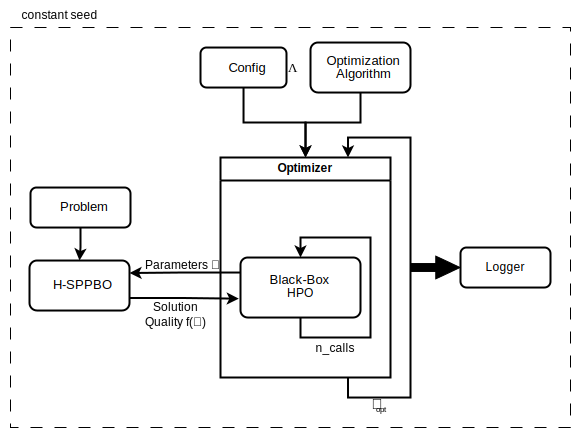
\includegraphics[width=0.8\textwidth]{optimizer_flow.svg}
	\caption{Visualization of the optimizer mode workflow.}
	\label{fig:optimizer-flow}
\end{figure}

\subsection{Experimentation Mode}
\label{chap:exp-mode}

The main task of the experimentation mode is to repeat multiple runs of a fixed metaheuristic, i.e. using only one parameter configuration. It is essentially a version of the run mode with options for multiple runs. Therefore, the inputs of this mode are also similar, with the parameter configuration $\mathbf{\lambda}$, problem parameters ($t, p, w_{di}$) and, additionally, the number of consecutive runs $r_\text{exp}$. The results for this mode are also logged in an averaged version, to easily plot the mean development of an algorithm across different random influences. That is why in this mode, the random seed is explicitly not set to a fixed value. See \cref{alg:xf-opt-run-exp} for an implementation template.


\begin{algorithm}
	\caption{XF-OPT/HSPPBO: Experimentation Mode}
	\label{alg:xf-opt-run-exp}
	\begin{algorithmic}
		\Require Number of runs $r_{\text{exp}}$, parameter configuration $\mathbf{\lambda}$, problem parameters ($t, p, w_{di}$)
		\State $\mathbb{L}  \gets $ \Call{InitLogger}{ } 
		\State $\mathcal{P}  \gets $ \Call{InitProblem}{$t,p,w_{di}$}
		\State $\mathcal{M}  \gets $ \Call{InitHSPPBO}{$\mathcal{P}, \mathbb{L}, \mathbf{\lambda}$}
		\For{$i=1$ to $r_{\text{exp}}$}
			\State $\mathbf{s} \gets $ \Call{Execute}{$\mathcal{M}, \mathcal{P}$}
			\State \Call{LogResults}{$\mathbb{L}, \mathbf{s}$}
		\EndFor
	\end{algorithmic}
\end{algorithm}



